% !TEX root = main.tex

\section{Experiments} \label{sec:experiments}

The confidence one can have on the encoders of the robot depends on several factors from actuators design to control strategies. in the legged locomotion case, this can also depend on the general design of the robot.
Thus during walking phases with humanoid robot HRP2, one can notice sliding phenomenon when the foot hits the ground. If this effect is not measured, their occurrences can turn to be a problem for navigation in unstructured environment. 
Furthermore, we cannot anticipate the sliding, meaning that we do not know what actually causes this to happen. 
In this context, we show that measuring this slide and getting a better estimation of both real trajectories and real position of the foot is possible with an IMU fixed on the sliding member, the foot of the robot in our case.

In order to get to that point, we first want to check whether our fusion method of both IMUs and odometer is able to get a correct estimation of one's foot during walking.
Then we show that using an IMU on the foot of the robot leads to a better estimation of the real position of the member compared to encoder based odometry.

We chose to use a low-cost IMU in our application to realize the feasibility of our method. For this purpose we selected the 
MPU6050 from Invensense combining both an accelerometer and a gyroscope and extensively used in the open source community.


%\textit{Keywords : low-cost IMU, MPU6050, experiment conditions, 1 KHz IMU} \\
%\textit{TODO : add factor graph for experiment visualization}

\subsection{Method}
\subsubsection{auto-calibration}

The parameters we need to calibrate for a correct integration are the biases on top of which we integrate the incoming data of the IMU.
The time varying property of the bias is a critical point to consider in order to avoid large deviations. This calibration is made possible
by dependencies of the delta pre-integration (${\Dp}(\bfa_b, \bw_b), {\Dv}(\bfa_b, \bw_b), {\Dq}(\bw_b)$). Fusing both odometer and IMU provides constraints on position and orientation parts of
the state vector. However, velocity is still not observable and is affected by the bias estimation. In the case of legged locomotion, we fix the observability problem by adding a zero velocity constraint when the foot is on the ground.

The initial orientation estimation is made possible by adding an absolute constraint on yaw part of the state vector, otherwise we would run into observability problems. \textbf{add figure here (graph)}

\subsection{Results}
\subsubsection{Trajectory reconstruction}

We check the feasibility of the trajectory reconstruction using a 1Khz IMU attached to one's foot tracked with a motion capture (MOCAP) system. The MOCAP is used to get odometry between zero-velocity phases, i.e. when the foot is on the ground,
and will be taken as the ground truth against which we compare the trajectory reconstruction.

We reproduce the movements the feet of a robot could have when it is walking. However, as shown in figures \textbf{add figure here}, the final optimal state
is not the expected one and acceleration biases are rapidly changing. The variation that we can see is not only due to some random walk and can be explained by the excitement of biases in a different axis.
As explained in \cite{roussillon2011rt}, in opposition to gyroscope biases, acceleration biases do not converge toward stable values during a motion exciting several axis of the sensor. 
This effect can be explained by time inconsistency meaning that we fail
to use the information of the entire motion to converge toward stable values as expected in the sensor model, but the problem may also be that the step motions do not use all the axis of the accelerometer as it should.

\begin{figure}[tb]
\begin{center}
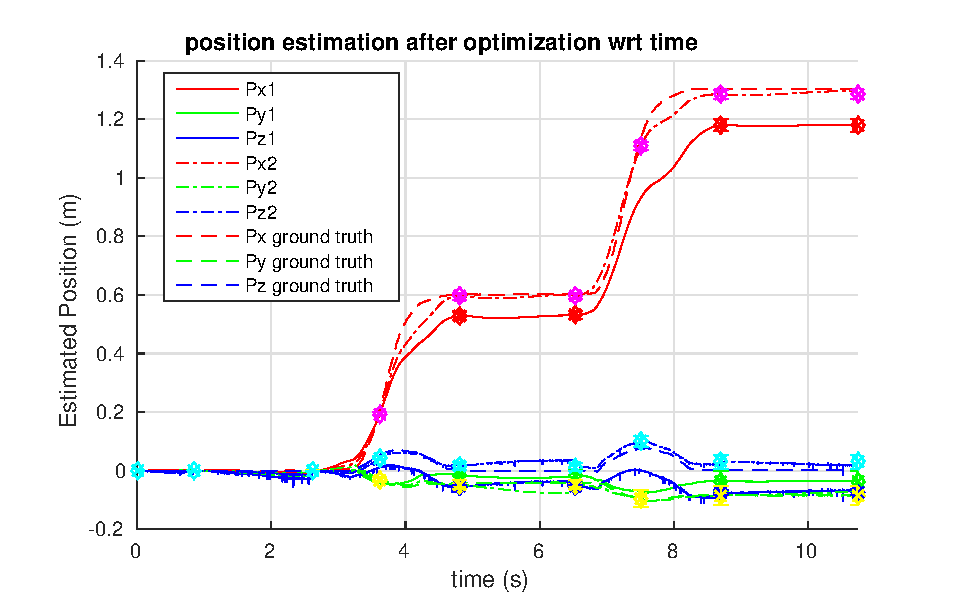
\includegraphics[scale=0.5]{figures/Result_position}
\par\vspace{4mm}
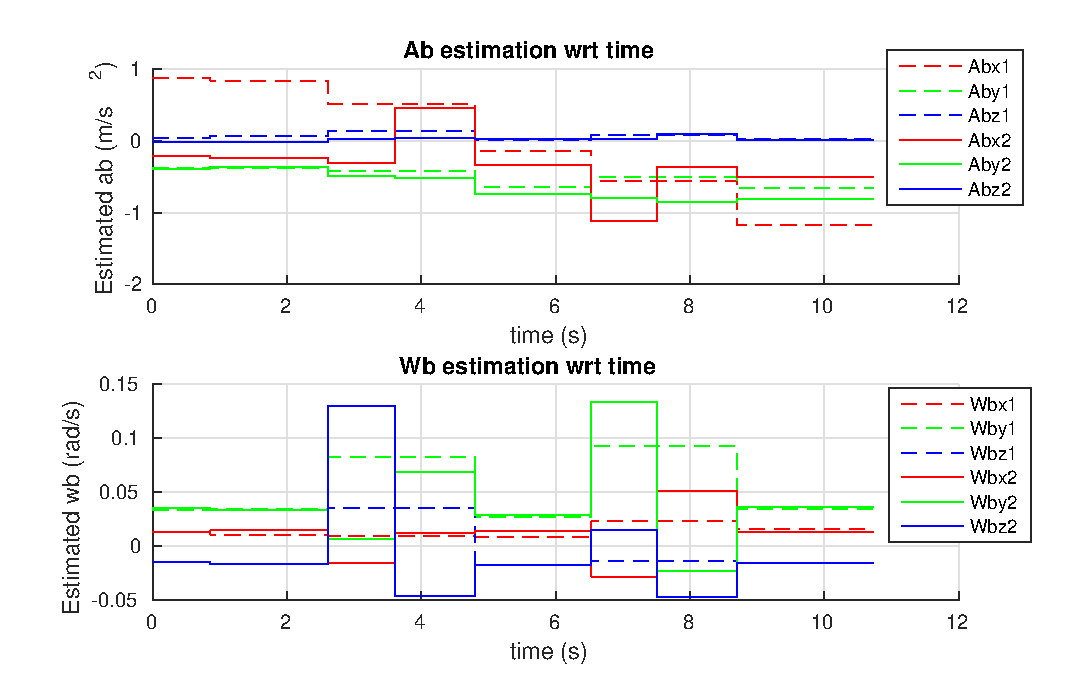
\includegraphics[scale=0.5]{figures/Result_bias}
\caption{ 
{\bf Top}: trajectory estimation during human walking with an IMU attached to a foot. Continuous, dashed and dashed-dot lines are respectively: mocap recorded ground truth, 
estimation with zero velocity constraints only, estimation using zero velocity constraint and 1 odometry measurement during foot's flying phase. odometry was here built from MOCAP information.
{\bf Bottom}: Evolution of corresponding estimated IMU biases 
}
\label{fig:forward_walk_IRI}
\end{center}
\end{figure}
We fix the trajectory estimation problem by adding odometry information during foot's flying phase. However, we cannot fix any other conditions making velocity and bias observation possible hence all parameters of the state vector are estimated.
This added KeyFrame reduces the integration time since last state optimization making bias random walk variation less critical on estimation. As we can see, results are much better and closer to MOCAP's ground truth as we could expect.

%TODO : process mocap experiments

\subsubsection{Legged-Locomotion's undesired behavior measurement}

We use the approach presented above in the case of the humanoid robot HRP2 to better estimate the trajectory of the foot. This also results in a better estimation of the pose of the robot using its kinematic chain. 
For this experiment, the robot is moving in open loop and some particularities are worth to be noted compared to previous experiment. 
The structure of the robot produces vibrations that are measured by the IMU, thus explaining the over noisy aspect of the data. The foot's flying phase is set to last 800 ms. The double support phase lasts only 20 ms, thus it is difficult to observe
even with the IMU working at 1 KHz because of the vibration it will measure on impacts.




%TODO experiment : step motion + complex rotation, followed by MOCAP


